\subsection{Trigger}
\label{sec:reco-el-triggers}

Events containing electrons are triggered on using ATLAS's three level trigger
system as described in~\sec{detector-trigger}. They are triggered on at L1 by
requiring two adjacent towers of calorimeter cells of size
\deltaetadeltaphi{0.1}{0.1} have an energy above a certain threshold. The towers
are used to identify a RoI for use at L2. At L2 fast calorimeter and tracking
algorithms are used. The calorimeter clustering uses a similar algorithm to in
the offline reconstruction as described in~\sec{reco-el-reco}, except that the
highest \et\ cell in the middle calorimeter layer of the RoI is used as a seed
rather than using a sliding window algorithm. Basic shower shape cuts on
the width of the shower in $\eta$ and the ratio of energy deposits in the
different calorimeter layers are
used to reject backgrounds. The EF uses the offline reconstruction and
identification algorithms described in~\sec{reco-el-reco}
and~\sec{reco-el-id}, although slightly looser cuts are applied to remain fully
efficient offline. 
%It uses some information from just outside the RoI.

The bandwidth dedicated to electron and photon triggers is approximately 30\% of the
total EF bandwidth. As instantaneous luminosity increased throughout 2011 and
2012 it was necessary to regularly tighten the triggers to keep the bandwidth at
an acceptable level~\cite{Monticelli:1450947}. At the start of 2011 the primary single electron trigger
has a threshold of 20 \gev. When the instantaneous luminosity exceeded
2\timestenpower{33}~\instlumiunit\ the threshold was increased to 22 \gev, and as
the luminosity further increased to 3\timestenpower{33}~\instlumiunit, the identification
requirements used at L2 and EF were tightened. The L1 thresholds were also
brought closer to the EF threshold, and varying L1 thresholds with $\eta$ were
introduced to account for varying material before the calorimeter. A hadronic
leakage cut was also introduced to further reduce the L1 rate. In 2012 the
threshold was further raised to 24 \gev, and a track isolation cut introduced at
EF, requiring that the total \pt\ of tracks surrounding the
electron's track in a cone of \deltaRlt{0.2} to have less than 10\% of the \pt\ of
the electron.

\subsection{Reconstruction}
\label{sec:reco-el-reco}

Electrons are reconstructed in the central region (\modetalt{2.5}) by searching
for EM calorimeter clusters and matching them to Inner Detector
tracks~\cite{ATL-PHYS-PUB-2011-006,Aad:2011mk}; this is
referred to as the \intro{standard} electron algorithm and is described below.
In the forward regions (\modetabetween{2.5}{4.9}) there is no Inner Detector
tracking, and electrons are reconstructed solely from calorimeter clusters; this
is also described below. The standard algorithm drops in efficiency at very
low \pt\
(a few \gev), but an alternative \intro{soft-e} algorithm can be used to recover
efficiency. This uses Inner Detector tracks as seeds, which it extrapolates into
the EM calorimeter and attempts to build clusters. It is not used in
this thesis so is not described in detail here.

\subsubsection{Standard Electron Reconstruction}

Reconstruction begins
with the construction of seed clusters in the EM calorimeter. These are formed from
calorimeter towers of size \deltaetadeltaphi{0.025}{0.025}, corresponding to the
size of cells in the second layer of the EM calorimeter. This
results in a grid of $200 \times 256$ towers. The energy
of the tower is the sum of the cells in all three layers
falling within the tower. Where cells are shared between more than one tower, the
energy is shared according the fractional overlap of the cell with each
tower. The seed cells are formed by sliding a
window of size \deltaetadeltaphi{0.075}{0.125} ($3 \times 5$ towers) over the
grid of towers and identifying local maxima with \etgt{2.5}. The position
of the cluster is taken to be the energy weighted $\eta$, $\phi$ barycentre of
cells in a window around the centre of the cluster. If two seeds are closer than
\deltaetadeltaphi{0.050}{0.050} only the one with higher \et\ is kept.

Electron candidates are then formed by matching Inner Detector tracks to the
seed clusters. If there is a reasonable agreement ($\Delta \eta <0.2$ and
$\Delta \phi <0.1$) between a track's co-ordinates (measured at the origin of the
track) and a cluster seed, the track is extrapolated from its last measurement point to
the middle layer of the EM calorimeter (TRT-only tracks are automatically
extrapolated). In $\eta$, the cluster is required to be within 
of$\Delta \eta <0.05$ of the track. In $\phi$, the cluster must be within $\Delta \phi < 0.1$ of
the track if it falls on the side towards which the track bends, or $\Delta
\phi < 0.05$ if it is on the opposite side. This asymmetry in the $\phi$
requirement is to
account for the fact that the electrons undergo heavy energy losses from
bremsstrahlung, due to the large amount of material in the Inner Detector, which
will tend to increase their bending,
particularly at high $\eta$. If a seed cluster matches to at least one track,
and electron candidate is formed. Seed clusters with no track matches are
considered as photon candidates. If several tracks match, tracks with hits with
silicon hits are preferred, and the one closest to the cluster in \deltaR\ 
is chosen. In the case of TRT-only tracks, only a matching in $\phi$ is required, 
due to the limited $\eta$ resolution in the TRT.

The clusters for electron candidates are then rebuilt, using a fixed rectangle of size 
\deltaetadeltaphi{0.075}{0.175} ($0.125 \times 0.125$) in the barrel (endcap),
again using a sliding window to find the local maximum. The cluster energy is
the sum of four components: the estimated energy deposits before the
calorimeter, the measured energy in the cluster, the estimated leakage laterally
into other calorimeter cells and the estimated longitudinal leakage behind the
EM calorimeter. The four terms are parameterised as a function of the measured
cluster energy in the pre-sampler (where it exists) and the measured energy in each of the three
calorimeter layers, based on detailed simulations of energy depositions in the
calorimeters and the dead material. At this stage additional calibrations are
applied to the electron energy based on measurements of \Zee\ and
\JPsiee~\cite{Aad:2011mk}. The energy of the electron is taken as the cluster
energy, and the direction as the track $\eta$ and $\phi$, providing the track
has sufficient silicon hits.

\subsubsection{Forward Electron Reconstruction}

Forward electrons are reconstructed from energy deposits in the calorimeter
only. \intro{Topological clusters}~\cite{Lampl:1099735} are formed by grouping neighbouring cells in three
dimensions. The topological clusters do not have a fixed size, but will depend
on the energy deposit and the clustering criteria used. Cells with a
signal versus noise significance above a high threshold $t_{\rm{seed}}$ are used as seeds.
Neighbouring cells with a signal significance above a lower threshold
$t_{\rm{cell}}$ are added to the cluster. The neighbours may act as
secondary seeds if they have signal significance above an intermediate threshold
$t_{\rm{neighbour}}$. For electron topological clusters $t_{\rm{seed}}$ is set
equal to $t_{\rm{neighbour}}$. The lower threshold at the cell perimeter ensures that
tails of showers are not discarded, while the higher thresholds for seeds and
neighbors suppress electronics and pile-up noise. The cells are split if they
contain more than one local maxima above a certain energy threshold. 

An electron candidate is constructed if the cluster has \etgt{5} and only a
small hadronic energy component. The energy
of the electron is taken as the sum of the energy of all cells belonging to the cluster,
corrected for energy loss before the calorimeter and lateral and for longitudinal
leakages. The direction of the forward electron is taken as the barycentre of the cells
belonging to the cluster.

\subsubsection{Improvements to electron reconstruction in 2011 and 2012}

By default the ATLAS track fitting assumes a pion hypothesis for the modelling
of material effects, as described in~\sec{tracking-std}. This does not account well for energy losses via
bremsstrahlung. Due to their small mass, these losses are most substantial for
electrons, and can have significant effects on their trajectories through the magnetic
field. The amount of material in the Inner Detector in terms of radiation lengths
$X_{0}$ is shown in~\fig{id-material}. The material budget in the Inner detector
is highly non uniform with, high concentration of material at high $\eta$ and at certain radii.
This leads to large variations of the reconstruction efficiency as a function of
$\eta$, and degradations in estimates of the track parameters. To this end the
deault ATLAS reconstruction was progressively improved in 2011 and 2012 to
better account for energy losses due to \brem\ in the Inner Detector.

\begin{figure}[h]
\centering
            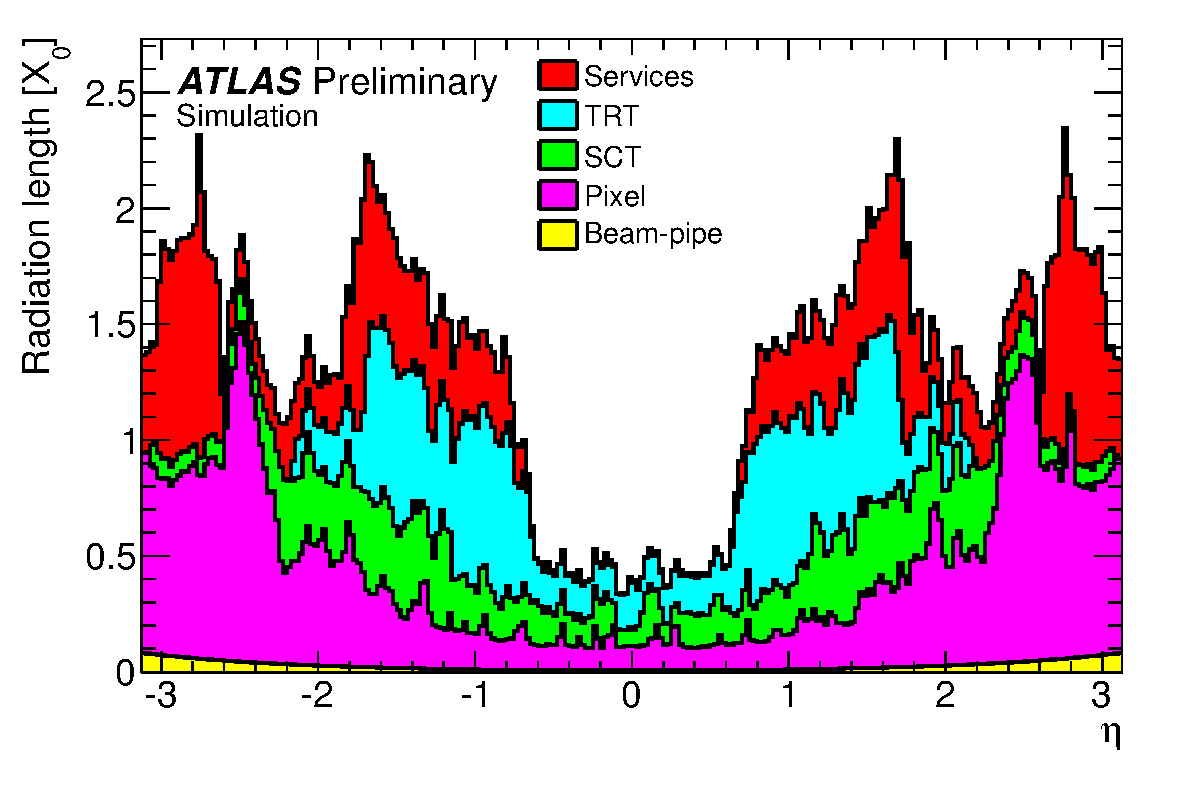
\includegraphics[width=0.8\textwidth]{id_material}
\caption{
Distribution of the Inner Detector material for each sub-detector as a
function of the pseudorapidity. The material of the Pixel and SCT detectors
includes passive material arising from electronics, cabling, cooling and
mechanical support. Figure from~\cite{ATLAS-CONF-2012-047}.}
\label{fig:id-material}
\end{figure}


The radiative loss of energy via \brem\ is highly non-Gaussian, and so is not
well modelled by the standard Kalman Filter, which can only incorporate Gaussian
noise terms. A non-linear extension of the
Kalman filter, the {\it Gaussian Sum Filter (GSF)}, has been
developed~\cite{Fruhwirth2003131,Atkinson:1448253}. It
approximates the PDF for energy loss from \brem\ as a weighted sum of Gaussian
components, and uses a separate Kalman Filter to process each one. For example,
one can consider the extrapolation of a measurement from a surface $k-1$ with state
described by $n_{k-1}$ components to surface $k$, where $\epsilon_{k}$ Gaussians
are used to describe the energy losses due to \brem\ between surfaces $k-1$ and
$k$. A separate Kalman Filter is applied to each of the $n_{k-1}$
components, for each of the $\epsilon_{k}$ noise terms, resulting in the state at
surface $k$ being described by $n_{k} = n_{k-1} \cdot \epsilon_{k}$ components.
At each layer the number of components is artificially reduced to a fixed number
by merging similar components,
in order to make the extrapolation computationally feasible.
Using the GSF filter allows for better pattern recognition by picking up hits
occurring after kinks in tracks caused by \brem, as well as improving the
resolution of the track parameters.

%\subsubsection{2011 Improvements}

For 2011 data taking, `brem-refitting' was applied to
reconstructed electron candidates~\cite{ATLAS-CONF-2012-047}. For technical reasons, it was not possible to
include the \brem\ recovery from the beginning of electron reconstruction.
Instead, electrons were reconstructed using the standard pion hypothesis
tracking and track cluster matching as described above. The tracks of these candidates were then refitted
using the GSF algorithm. All tracks with \ptgtMeV{400} and \modetalt{2.5} assigned to
electron candidates were refitted, the cluster-track matching re-run
using the collection of refitted tracks, and the rest of the electron reconstruction
chain re-run using these refitted candidates. This led to the best matches between
cluster and track changing in approximately 5\% of cases at high pseudo-rapidity (0.8 \%
overall). However, since it was only possible to run the refitting on tracks
already associated to electron clusters using the standard tracking, the full
benefit of using GSF was not gained as many tracks with significant energy loss
from \brem\ would not be reconstructed successfully by the standard tracking and
thus could not be re-fitted. For this reason the brem-refitting did not
significantly improve the reconstruction efficiency, but did significantly
improve the resolution of track parameters in the bending plane such as \dzero, \dzerosig,
$\phi$ and \qoverp. For example, \fig{d0Sig-gsf} shows the impact parameter
significance (\dzerosig) distribution with and without the GSF refit. 

\begin{figure}[h!]
\centering
            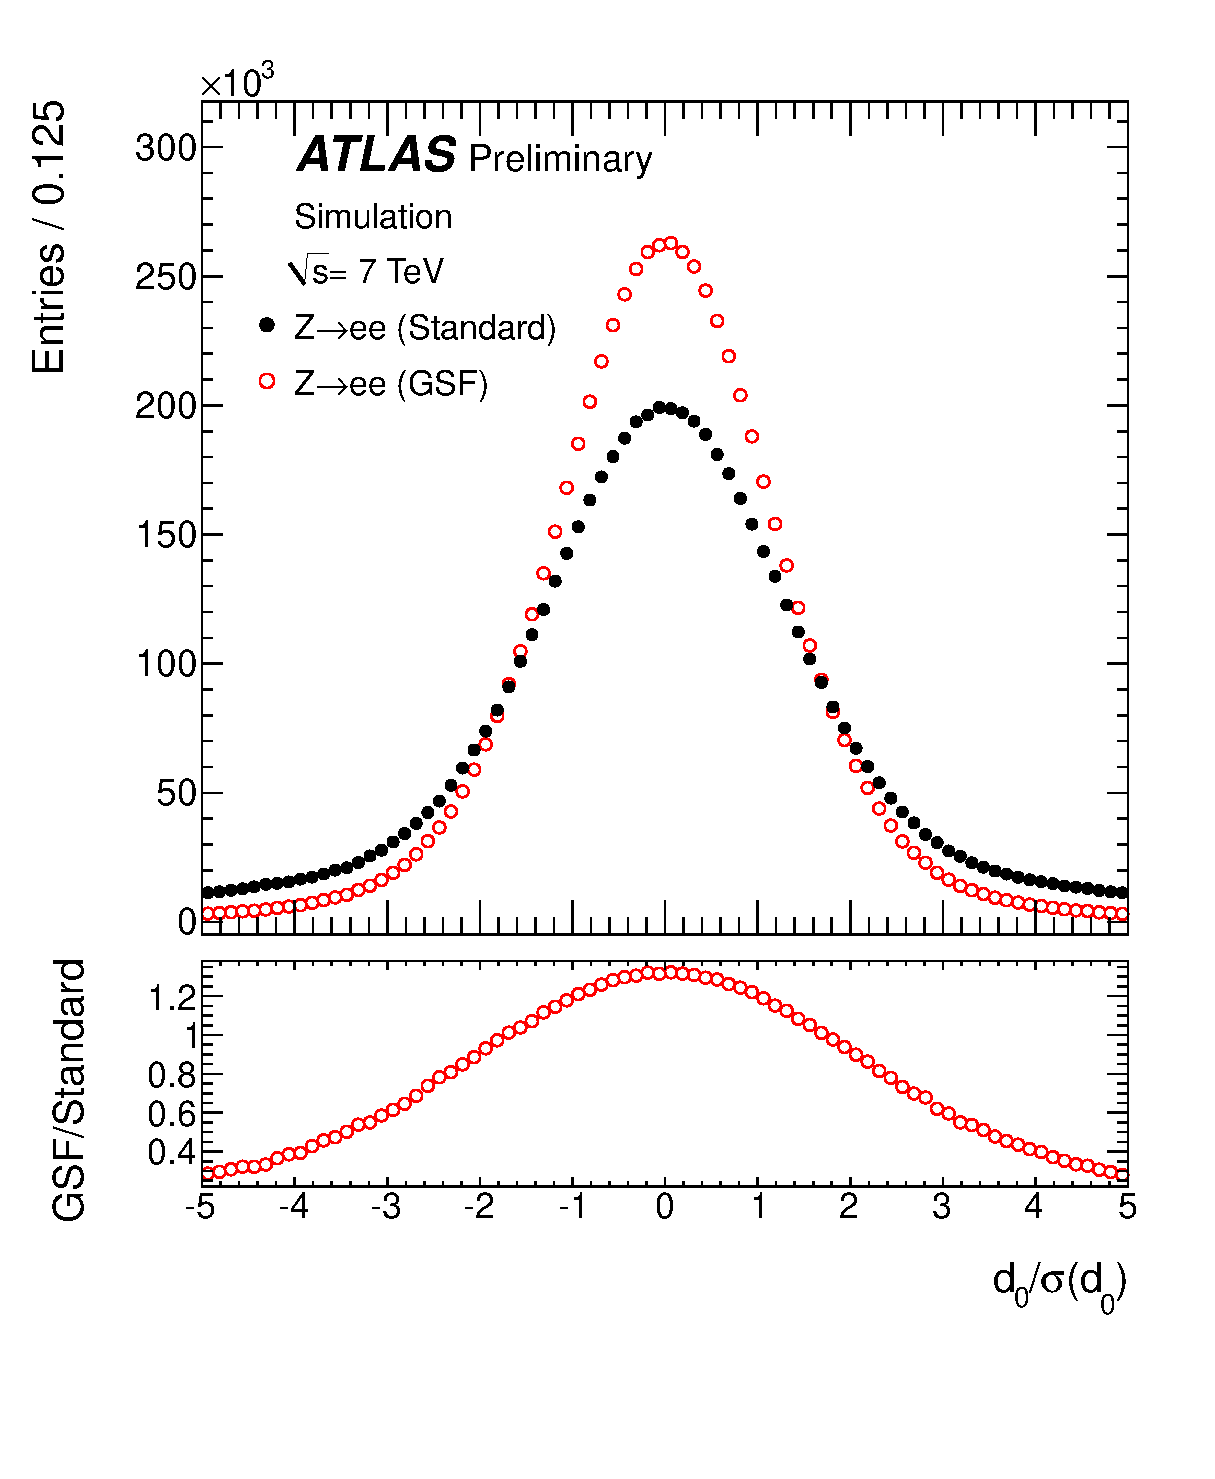
\includegraphics[width=0.7\textwidth]{d0Sig_gsf}
\caption{
Distribution of the simulated transverse impact parameter significance for GSF (open
red) and standard (solid black) electrons from \Z-boson decays. 
%The bottom plots show the ratio of the entries of the GSF and standard
%electrons per bin
Figure from~\cite{ATLAS-CONF-2012-047}.}
\label{fig:d0Sig-gsf}
\end{figure}

%\subsubsection{2012 Improvements}

In 2012, improvements were made to all stages of the electron reconstruction
chain, from the initial tracking pattern recognition through to the track
cluster matching~\cite{HSG2:1456228}. 

Since the GSF tracking takes approximately 10 times more time to
run than the standard Kalman filter, it is not feasible to fit all tracks using
the GSF when doing the initial pattern recognition and track finding (see~\sec{tracking-std}). 
Additionally, the use of such a filter with electron hypothesis would
negatively affect non-electron tracks. Instead, the effects of \brem\ on
electron tracks are crudely modelled at the initial pattern recognition by allowing for 30\% energy loss at each surface for tracks with
momentum above 1 \gev. In order to avoid degrading non-electron tracks, this allowance is only made in regions of interest in a
cone of \deltaRlt{0.3} around EM calorimeter clusters. 

The global \chisquared\
fitter was also improved to allow for electron hypothesis tracks. Tracks
rejected due to low \chisquared\ at the ambiguity resolution stage in a RoI were
refitted using a modified `electron hypothesis' global \chisquared\ fitter. This
attempts to find the layer with the most significant \brem\ energy loss, then
reruns the fit with only an energy loss term for the most significant \brem\
loss. The advantage of this over the standard \chisquared\ fit, which allows
includes an energy loss term for each layer, is that in the latter approach the
electron momentum tends to be overestimated as all of the energy loss terms tend
to take the average energy loss value, rather than correctly identifying one layer with large
energy loss. The modified \chisquared\ fitter gives a significant improvement in the track
parameter resolution, giving an improvement almost as great as using the more
sophisticated GSF algorithm, but running in approximately one tenth of the time.

At this stage, there will still be a number of tracks which had large energy
losses from \brem\ and were consequentially badly fitted. A refit using the GSF
fitter described above is thus carried out for all tracks loosely matched to an
EM calorimeter cluster. Two forms are matching are carried out: the first
(\deltaR) between the
track parameters extrapolated to the second layer of the calorimeter and the
barycentre of the calorimeter cluster, and the second (\deltaR$^{\rm{rescaled}}$) where the track momentum is
scaled to the cluster energy before extrapolating the track to the calorimeter.
Loose cuts are made on \deltaR\ and \deltaR$^{\rm{rescaled}}$, with the cuts on
\deltaR$^{\rm{rescaled}}$ being slightly tighter.
Tracks which match under either of the two scenarios are refitted; the latter
category aims to select tracks with low momentum that have suffered large
\brem\ and would otherwise be missed. The final matching of the refitted tracks
to the clusters and selection of the best match is also improved; again both the
original \deltaR\ and the \deltaR$^{\rm{rescaled}}$ after scaling the track
momentum to the cluster
energy are computed. Tracks with Pixel detector hits are preferred. If there are
more than two tracks with Pixel hits the one with the smaller
\deltaR$^{\rm{rescaled}}$ is preferred, providing they are well enough
separated in \deltaR$^{\rm{rescaled}}$, otherwise the one with smaller \deltaR\
is chosen.

Overall these improvements increase the electron reconstruction efficiency by
$\sim1\%$ in the calorimeter barrel and $\sim5\%$ in the calorimeter endcaps.
For low \et\ electrons (\etlt{20}) the improvement is up to 8\%.

\subsubsection{Electron Reconstruction Efficiencies}

\begin{figure}[h]
\centering
	\subfigure[]{
            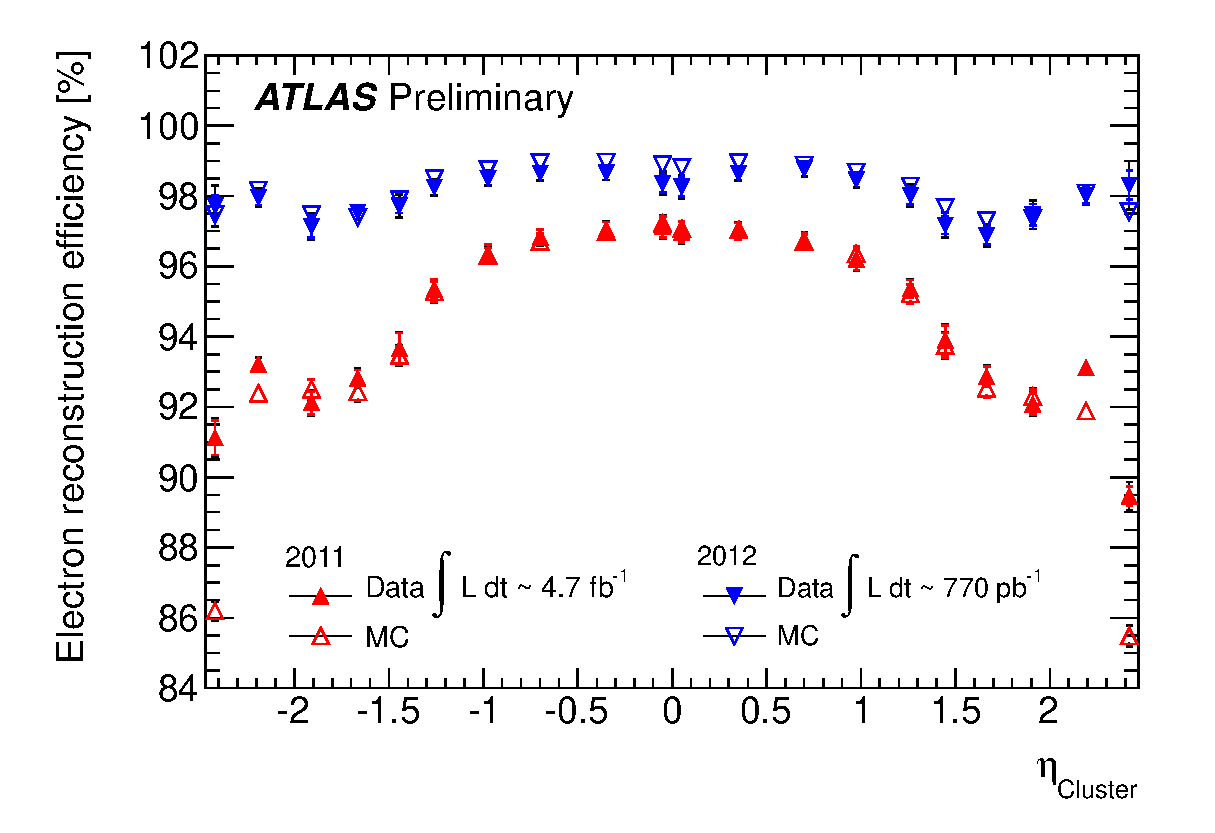
\includegraphics[width=0.47\textwidth]{ElRecoEffEtaBin2011_2012}
        }
	\subfigure[]{
            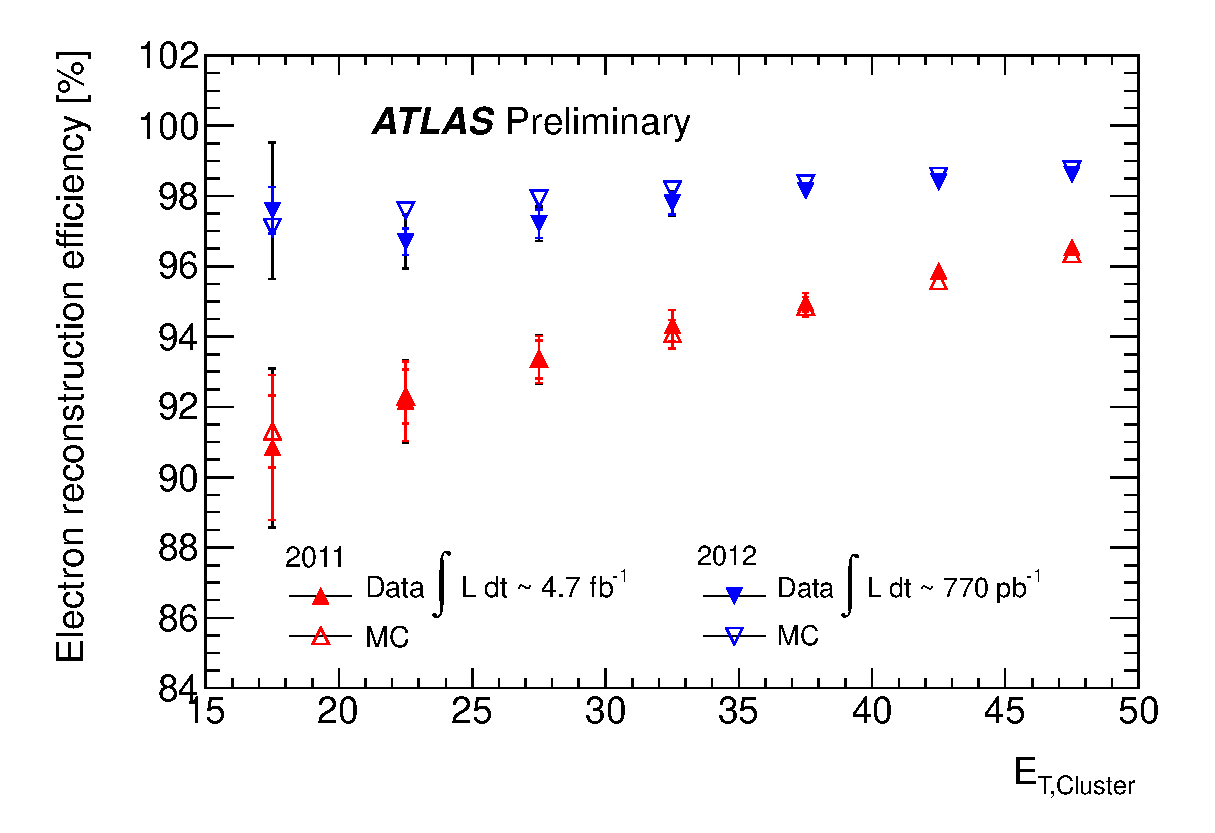
\includegraphics[width=0.47\textwidth]{ElRecoEffPtBin2011_2012}
        }
\caption{Electron reconstruction efficiency in 2011 and 2012 as a function of (a) the cluster
$\eta$ and (b) the cluster \et. The solid coloured points show the efficiency
observed in data whilst the open points show the simulated efficiency in
Monte-Carlo. Figures from~\cite{ElectronEfficiency2012}.}
\label{fig:el-reco-eff}
\end{figure}

\subsection{Identification}
\label{sec:reco-el-id}

The electron candidates reconstructed as described in the previous section will
contain a high contamination from jets faking electrons, non-isolated electrons
from decays in jets and electrons from photon conversions. In order to identify prompt isolated photons a
cut based identification is used. Cuts are made on variables relating to the
shape of the electromagnetic shower in the calorimeter, the quality of the Inner Detector track, the
track-calorimeter matching and particle identification information from the
TRT. The cuts were optimised using a multivariate analysis program (TMVA), in 10 bins
of cluster $\eta$ and 11 bins of cluster \et\ from 5 \gev\ to $>80$ \gev.
Three reference sets of cuts are used, denoted \loose, \medium\ and \tight,
designed to give progressively greater background rejection, at the cost of
signal efficiency. The expected jet rejections (from simulation) of the three points are 500, 5000
and 50000 respectively~\cite{ATL-PHYS-PUB-2011-006}.

In order to maintain manageable trigger rates with increased instantaneous
luminosity, the original \loose, \medium\ and \tight\ were re-optimised in order
to increase background rejection. The new working points are denoted \loosePP,
\mediumPP\ and \tightPP. In 2012, the identification was further re-optimised to
prevent drops in efficiency in events with high pileup of up to 20\%. 

In both 2011 and 2012 \loosePP\ cuts on shower shape variables in the first and
second layers of the EM calorimeter, leakage into the hadronic
calorimeter, track quality in the silicon detectors and loose track cluster
matching. The variables cut on are as follows:

\subsubsection{\loosePP\ Requirements}

\begin{itemize}

    \item {\bf Shower Shapes:} cuts are made on the following shower shape
    variables:

    \begin{itemize}
        \item Hadronic leakage, \Rhad, the ratio of \et\ in the first layer of
        the hadronic calorimeter to the \et\ of the EM cluster. In the range
        \modetabetween{0.8}{1.37} the \et\ of the full hadronic calorimeter is
        used, to compensate for the crack between the barrel and extended barrel
        of the tile calorimeter.
        \item Lateral width of the shower in the second layer of the EM
        calorimeter, \wetatwo.
        \item Ratio of the energy difference between with the largest and second
        largest energy deposit in the first layer of the EM calorimeter over the
        sum of their energies, \Eratio.
        \item Total width of the shower in the first layer of the EM
        calorimeter, \wstot.
    \end{itemize}

    \item {\bf Silicon Hits:} at least 7 hits in the silicon detectors, of which at
    least one must be in the pixel detector. This ensures good track quality and
    rejects backgrounds from conversions or Dalitz-decays.
    \item {\bf Track-Cluster matching:} a loose matching in $\eta$ is applied,
    requiring \deltaetalt{0.015}
\end{itemize}

The shower shape variables \Reta\ and \Rhad\ are particularly susceptible to
pileup since they sample a large area of the calorimeter. Cuts on these
variables were therefore
loosened in 2011 with respect to 2012, reducing the rejection power of \loosePP\
by about 20\%.

\subsubsection{\mediumPP\ Requirements}

All \loosePP\ cuts are required to be passed, and in addition:

\begin{itemize}
    \item {\bf Shower Shapes:} the shower shape cuts made in \loosePP
    (\Reta, \Rhad, \wetatwo, \Eratio, \wstot) are made at tighter values. For
    2012, the cuts on \Reta\ and \Rhad\ were loosened with respect to 2011, and
    made at the same value as for \loosePP, whilst the cuts on  \wetatwo, \Eratio\ and
    \wstot\ were tightened with respect to 2011.

    \item {\bf Track-Cluster matching:} a tighter matching in $\eta$ is applied,
    requiring \deltaetalt{0.005}.

    \item {\bf Impact Parameter:} require that the electron's track has a
    transverse impact parameter \dzero $<$ 5 mm.

    \item {\bf Silicon Hits:} stricter requirements are made on hits in the
    silicon detectors. Require that there is at least one hit in the b-layer for
    \modetalt{2.01} (\modetalt{2.37} in 2012). In 2011, at least 1
    Pixel hit is required for \modetalt{2.01} and at least two for
    \modetagt{2.01}. For 2012, two Pixel hits are required in all bins.

    \item {\bf Fraction in third calorimeter layer \fthree:} for 2012 a cut on the
    fraction of the shower energy deposited in the third layer of the EM
    calorimeter was added to compensate for the loosening of the cuts in the
    first layer of the calorimeter. This cut is only applied for \etlt{80}, since
    the depth of the EM shower and hence leakage into the third layer increases
    with energy.

    \item {\bf TRT High Threshold Hits} A loose requirement is made on the
    fraction of high-threshold (HT) hits from transition radiation photons in the
    TRT detector (see~\sec{Detector-TRT}).

\end{itemize}

\subsubsection{\tightPP\ Requirements}


All \mediumPP\ cuts are required to be passed, and in addition:

\begin{itemize}
    \item {\bf Shower Shapes:} cuts on shower shape variables are made at equal
    or tighter values to those for \mediumPP. As for \mediumPP,
    the cuts on \Reta\ and \Rhad\ were loosened in 2012 with respect to 2011, 
    whilst the cuts on  \wetatwo, \Eratio\ and
    \wstot\ were tightened.

    \item {\bf Track-Cluster matching:} a cluster matching in $\phi$ is added,
    requiring \deltaphilt{0.02}, and cuts are made on the ratio of the cluster
    energy to the track momentum, \Eoverp.

    \item {\bf Impact Parameter:} the
    transverse impact parameter cut is tightened to \dzero\ $<$ 1 mm.

    \item {\bf Silicon Hits:} stricter requirements are made on hits in the
    silicon detectors, requiring that there is at least one hit in the b-layer for
    all $\eta$, and, in 2012, at least 2 hits in the Pixel detector for all
    $\eta$.

    \item {\bf Conversion Rejection:} candidates matched to reconstructed photon
    conversions are rejected.

\end{itemize}

\subsubsection{Forward Electron Identification}

Since in the forward region there is no tracking from the Inner Detector,
identification in the forward region must rely on calorimeter shower shape
variables alone. A god discrimination between electrons and hadrons may be made
due to the fine transverse and longitudinal segmentation of the calorimeter, but
it is not possible to distinguish electrons and photons in the forward regions.
Two reference sets of cuts are defined for forward electrons, \loose\ and
\tight.

\subsubsection{Forward \loose\ Requirements}

Cuts are made on the following variables:

\begin{itemize}
    \item {\bf Shower depth, $\lambda_{\rm centre}$} the distance of the shower
    barycentre from the front face of the calorimeter along its axis.  
    \item {\bf Longitudinal Second Moment, $\langle \lambda^2 \rangle$} the second
    moment\footnote{The $n^{\rm th}$ moment is defined as $\langle x^n \rangle =
    \frac{\sum_{i} E_i x^n_i}{\sum_{i} E_i}$ where $i$ runs over all cells in the
    cluster.} of the distance of each cell to
    the shower barycentre in the longitudinal direction.  
    \item {\bf Transverse Second Moment, $\langle r^2 \rangle$} the second moment of the 
    distance of each cell to the shower barycentre in the transverse direction.
\end{itemize}

\subsubsection{Forward \tight\ Requirements}

All of the \loose\ cuts are required to be passed, an in addition cuts are made
on the following variables:

\begin{itemize}
    \item {\bf Fraction Fraction of cluster energy in the most energetic cell,
    $f_{\rm max}$.}
    \item {\bf Normalized lateral moment, $\frac{w_{2}}{w_{2} + w_{\rm max}}$} where
    $w_{2}$ is the second moment of $r_{i}$ setting $r_{i} = 0$ for the two most
    energetic cells and $w_{\rm max}$ is the second moment of $r_{i}$ setting
    $r_{i} = 4$ cm for the two most energetic cells and $r_{i} = 0$ for the
    remaining cells.
    \item {\bf Normalized longitudinal moment, $\frac{l_{2}}{l_{2} + l_{\rm
    max}}$}
    where, similarly to the normalised longitudinal moment, 
    $l_{2}$ is the second moment of $\lambda_{i}$ setting $\lambda_{i} = 0$ for the two most
    energetic cells and $l_{\rm max}$ is the second moment of $\lambda_{i}$ setting
    $\lambda_{i} = 10$ cm for the two most energetic cells and $\lambda_{i} = 0$ for the
    remaining cells.
\end{itemize}

\subsubsection{Electron Reconstruction Efficiencies}

\begin{figure}[h]
\centering
	\subfigure[]{
            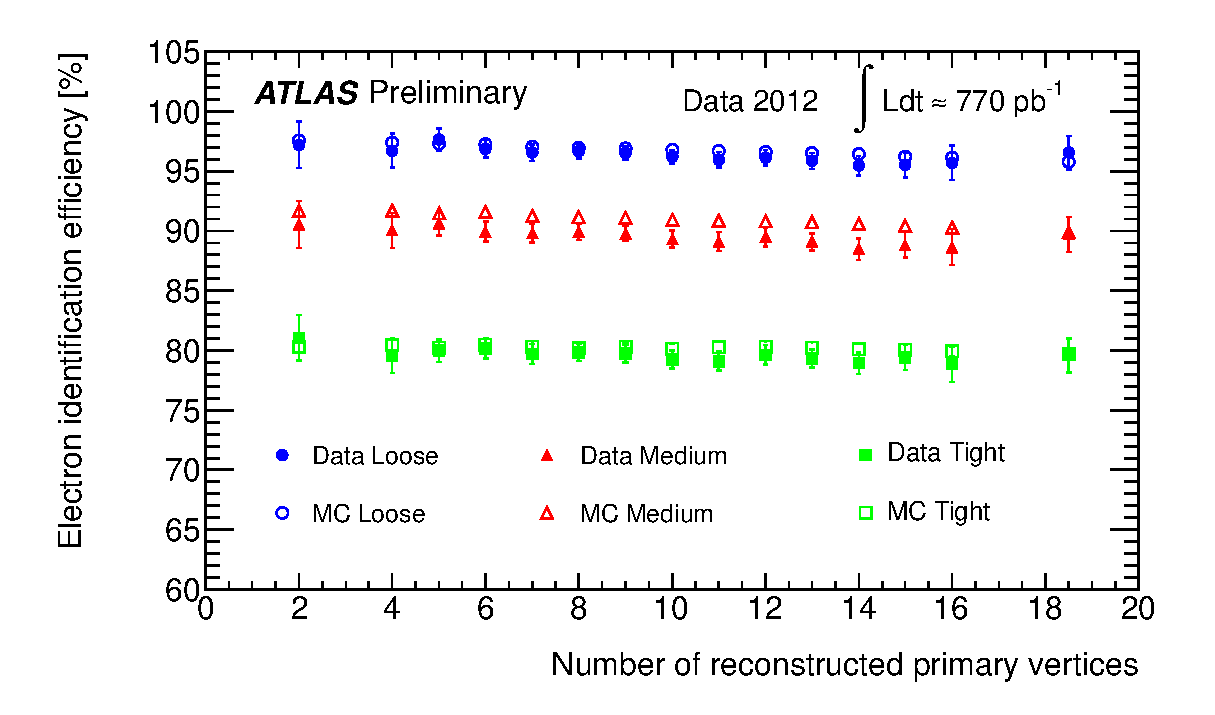
\includegraphics[width=0.47\textwidth]{ElIdEff_NPV_2012}
        }
	\subfigure[]{
            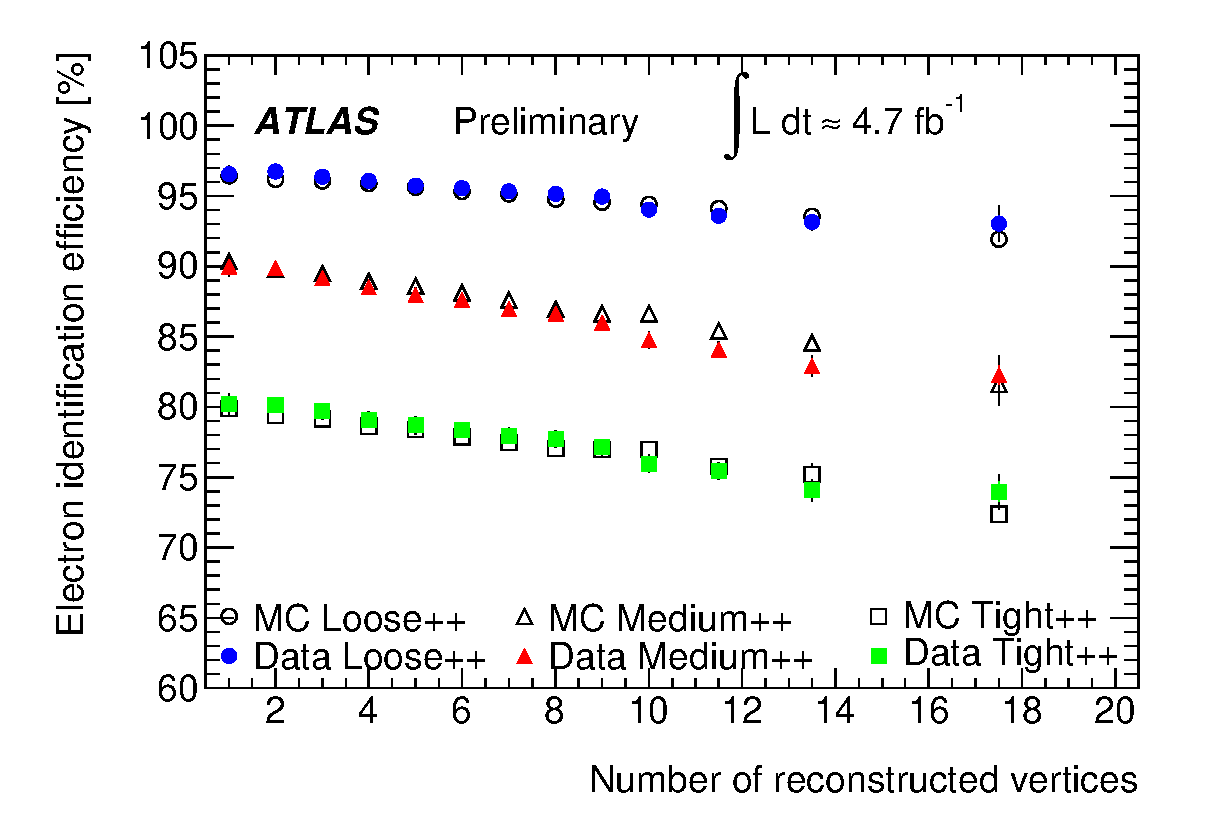
\includegraphics[width=0.47\textwidth]{Eff_PP_pileup2011}
        }
	\subfigure[]{
            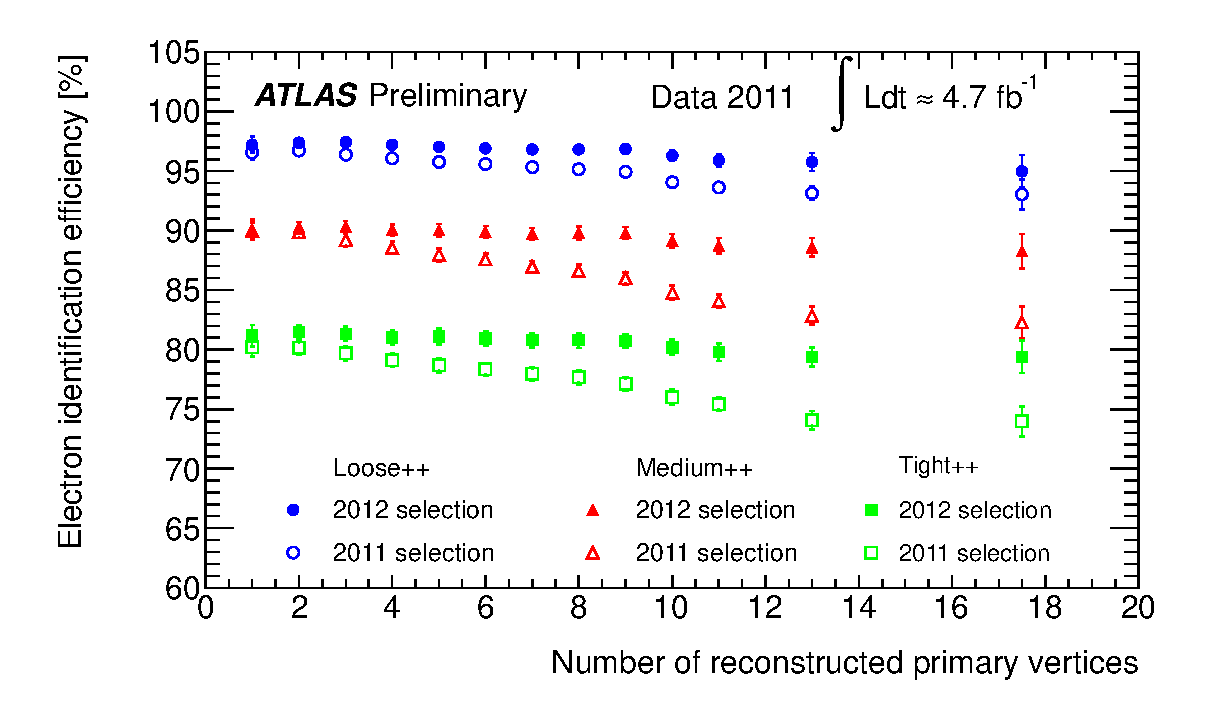
\includegraphics[width=0.47\textwidth]{data_effPP_vs_pvx_2011_2012}
        }
	\subfigure[]{
            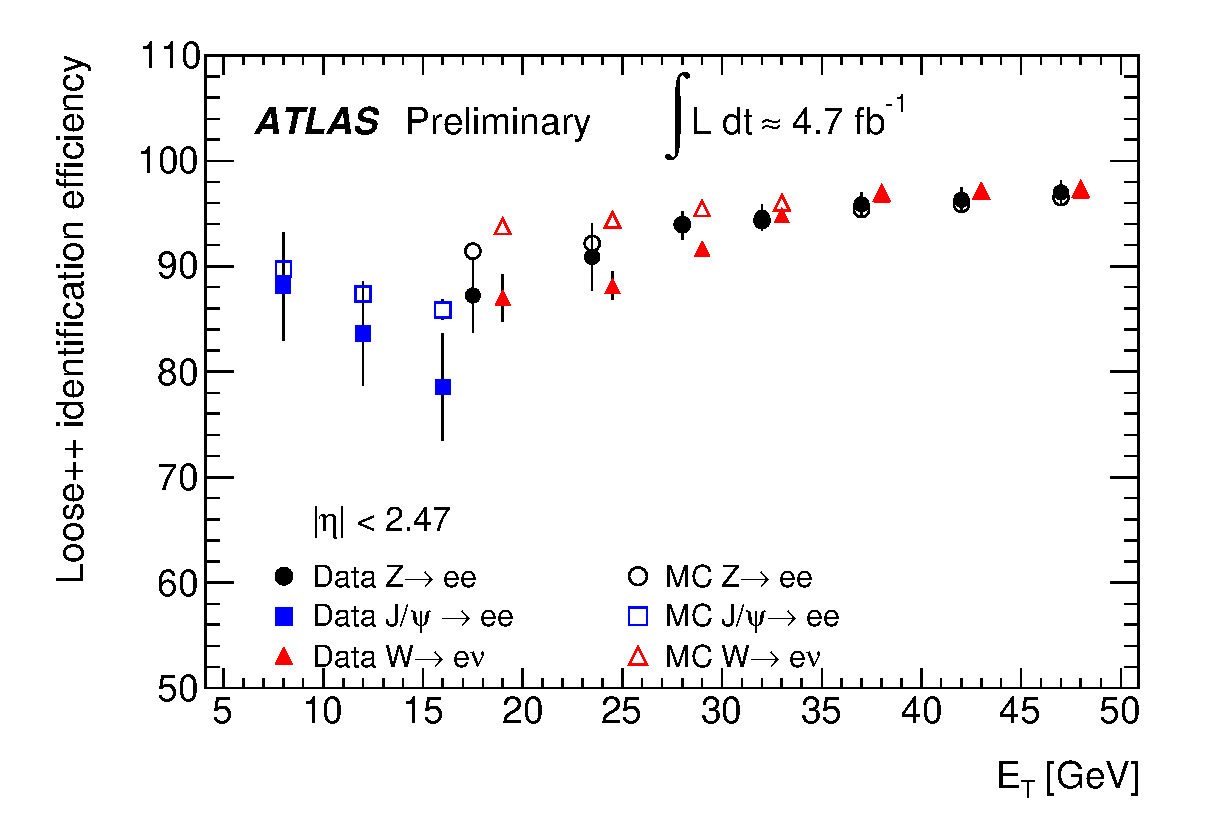
\includegraphics[width=0.47\textwidth]{ElLoosePPEfficiencyPt2011}
        }
\caption{Electron reconstruction efficiency in 2011 and 2012 as a function of (a) the cluster
$\eta$ and (b) the cluster \et. The solid coloured points show the efficiency
observed in data whilst the open points show the simulated efficiency in
Monte-Carlo. Figures from~\cite{ElectronEfficiency2012}.}
\label{fig:el-reco-eff}
\end{figure}


%The cluster reconstruction efficiency is very efficient for electrons:
